

\documentclass{article}
\usepackage[utf8]{inputenc}
\usepackage{authblk}
\usepackage{setspace}
\usepackage[margin=1.25in]{geometry}
\usepackage{graphicx}
\graphicspath{ {./figures/} }
\usepackage{subcaption}
\usepackage{amsmath}
\usepackage{lineno}
\linenumbers


%%%%%% Bibliography %%%%%%
% Replace "sample" in the \addbibresource line below with the name of your .bib file.
\usepackage[style=nejm, 
citestyle=numeric-comp,
sorting=none]{biblatex}
\addbibresource{sample.bib}

%%%%%% Title %%%%%%
% Full titles can be a maximum of 200 characters, including spaces. 
% Title Format: Use title case, capitalizing the first letter of each word, except for certain small words, such as articles and short prepositions
\title{Master's timeline}

%%%%%% Authors %%%%%%
% Authors should be listed in order of contribution to the paper, by full first name, then middle initial (if any), followed by last name and separated by commas.
% Please do not use initials for first names. If you use your middle name as a full name, use an initial for the first name and spell out your full middle name.
% Use a superscript asterisk (*) to identify the corresponding author and be sure to include that person’s e-mail address. Use symbols (in this order: †, ‡, §, ||, ¶, #, ††, ‡‡, etc.) for author notes, such as present addresses, “These authors contributed equally to this work” notations, and similar information.
% You can include group authors, but please include a list of the actual authors (the group members) in the Supplementary Materials.
\author[]{Christophe Rouleau-Desrochers}


%%%%%% Affiliations %%%%%%
%%%%%% Date %%%%%%
% Date is optional
\date{19 September, 2024 \\ (started on the plane from Edmonton to Montreal)}

%%%%%% Spacing %%%%%%
% Use paragraph spacing of 1.5 or 2 (for double spacing, use command \doublespacing)

\onehalfspacing

\begin{document}

\maketitle

%%%%%% 2024 %%%%%%
\section{2024}
\subsection {October 2024}
\begin {itemize}
	\item \textbf{Literature review}: read 20 papers
	\item \textbf{Fuelinex}: senescence data collection
	\item \textbf{Side project 1}: Get trainings done for sanding 
	\item \textbf{Side project 1}: Sand all cookies
	\item \textbf{Side project 1}: Figure out which trees for tree spotters and ask for permits
	\item \textbf{Side project 2}: Dendrometers troubleshooting
	\item \textbf{Master's steps}: Discuss committee members with Lizzie 
	\item \textbf{Master's steps}: Update CGS-M and send 1st version to Lizzie
	\item \textbf{Master's steps}: Fill out the following form for 18 credit thesis https://ubc.ca1.qualtrics.com/jfe/form/SV_4ITKPKPRc50A1uK
\end {itemize}

\subsection {November 2024}
\begin {itemize}
	\item \textbf{Literature review}: read 30 papers
	\item \textbf{Side project 1}: Finish sanding cookies
	\item \textbf{Side project 1}: Scan all cookies
	\item \textbf{Master's steps}: Finish application for CGS-M and submit
	\item \textbf{Master's steps}: Schedule comittee for somewhere in the spring
\end {itemize}

\subsection {December 2024}
\begin {itemize}
	\item \textbf{Literature review}: read 30 papers
	\item \textbf{Fuelinex}: add nutrients to control trees
	\item \textbf{Side project 1}: cookie cross dating and tree ring analysis
	\item \textbf{Master's steps}: Class 1 completed: Biomathematics
\end {itemize}

%%%%%% 2025 %%%%%%
\section {2025}
\subsection {January 2025}
\begin {itemize}
	\item \textbf{Literature review}: read 30 papers
	\item \textbf{Fuelinex}: tree repotting
	\item \textbf{Fuelinex}: nutrient wash off of all trees
	\item \textbf{Master's steps}: start outline the chapters in my research proposal
\end {itemize}

\subsection {February 2025}
\begin {itemize}
	\item \textbf{Master's steps}: prepare committee meeting
	\item \textbf{Fuelinex}: diameter and height data collection
\end {itemize}

\subsection {March 2025}
\begin {itemize}
	\item \textbf{Master's steps}: first comitee meeting
\end {itemize}

\subsection {April 2025}
\begin {itemize}
	\item \textbf{Master's steps}: Class 2 completed: Bayesian
	\item \textbf{Master's steps}: Class 3 completed: Dolph's quantitative methods class
\end {itemize}

\subsection {May 2025}
\begin {itemize}

\end {itemize}

\subsection {June 2025}
\begin {itemize}
	\item \textbf{}
\end {itemize}

\subsection {July 2025}
\begin {itemize}
	\item \textbf{}
\end {itemize}

\subsection {August 2025}
\begin {itemize}
	\item \textbf{}
\end {itemize}

\subsection {September 2025}
\begin {itemize}
	\item \textbf{}
\end {itemize}

\subsection {October 2025}
\begin {itemize}
	\item \textbf{}
\end {itemize}

\subsection {November 2025}
\begin {itemize}
	\item \textbf{}
\end {itemize}

\subsection {December 2025}
\begin {itemize}
	\item \textbf{}
\end {itemize}


\subsection {Summer}
\begin {itemize}
	\item Fuelinex: bud burst and shoot elongation
	\item Fuelinex: start analysis
\end {itemize}

\subsection {Autumn}
\begin {itemize}
	\item Fuelinex: biomass data collection
	\item Fuelinex: tree rings analysis 
	\item Start writting thesis 
	\item Class 4: last class (TBD)
	\item Semester abroad (??)
\end {itemize}

%%%%%% 2026 %%%%%%
\section {2026}
\subsection {Winter}
\begin {itemize}
	\item Finish writting thesis
	\item Finish analysis
	\item Submit first draft
\end {itemize}

\subsection {Summer}
\begin {itemize}
	\item Thesis defense
\end {itemize}

%%%%%%

%%%%%\subsection{Experimental Design}
%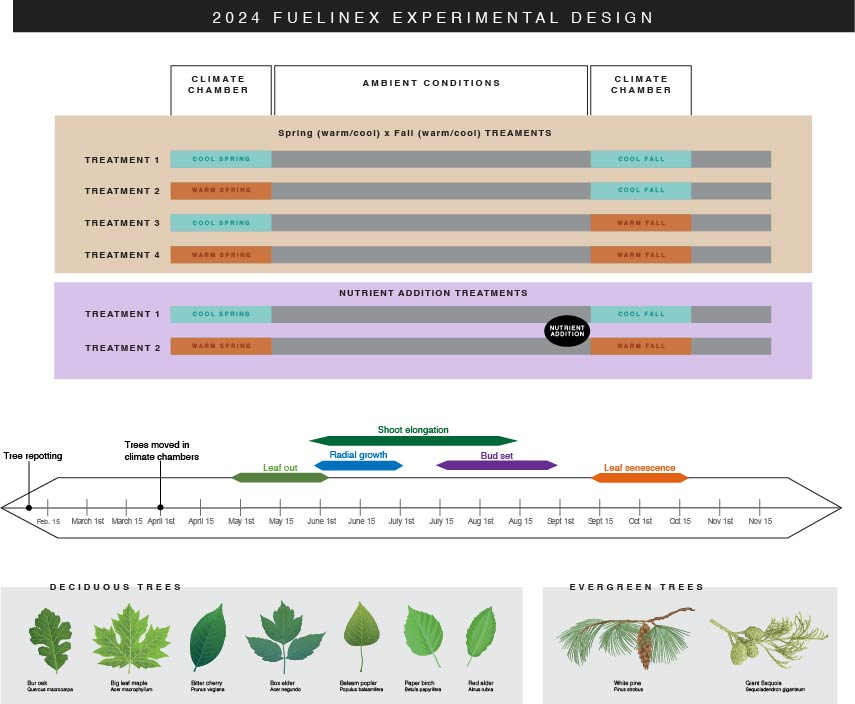
\includegraphics[]{../experimental_design/Fuelinex_Design_V4.jpg}

\end{document}
